\documentclass[a0paper]{sciposter}
\RequirePackage[utf8,utf8x]{inputenc}
\usepackage{url}
\usepackage{multicol}
\usepackage{graphicx}
\usepackage{color}
\usepackage{subfig}
\usepackage[dvips,dvipdfm,top=4cm,bottom=10cm,left=4cm,right=8cm]{geometry}

% usar para termos estrangeiros
\newcommand{\eng}[1]{\textit{#1}}

\newcommand{\rameau}[1]{\textit{Rameau}}

\renewcommand{\papertype}{a0paper}
\renewcommand{\fontpointsize}{25pt}

% \setlength{\paperwidth}{85cm}
% \setlength{\paperheight}{127cm}
% \renewcommand{\setpspagesize}{
%   \ifthenelse{\equal{\orientation}{portrait}}{
%     \special{papersize=85cm,127cm}
%     }{\special{papersize=127cm,85cm}
%     }
%   }

\definecolor{SectionCol}{rgb}{1,1,1}
\definecolor{BoxCol}{rgb}{.230,.230,.76}

\def\abovestrut#1{\rule[0in]{0in}{#1}\ignorespaces}
\def\belowstrut#1{\rule[-#1]{0in}{#1}\ignorespaces}

\def\abovespace{\abovestrut{0.20in}}
\def\aroundspace{\abovestrut{0.20in}\belowstrut{0.10in}}
\def\belowspace{\belowstrut{0.10in}}

\title{Functional Harmonic Analysis and Computational Musicology in
  Rameau}

\author{Alexandre Tachard Passos, Marcos Sampaio, Pedro Kröger,
  Givaldo de Cidra}

\institute{Genos---Computer Music Research Group \\
Federal University of Bahia (UFBA). Salvador, Brazil}

\email{pedro.kroger@gmail.com}

% The following commands can be used to alter the default logo settings
% \leftlogo[.7]{figs/ufba-logo}{  % defines logo to left of title (with scale factor)
% \rightlogo[1.1]{figs/capes-logo}  % same but on right

\begin{document}

\bibliographystyle{plain}

\conference{\Large \textbf{XII SBCM --- 2009
    \hfill \textsf{GENOS Research Group}}}

\maketitle

\begin{multicols}{2}

\section{About}

Rameau is an open-source system for automatic harmonic analysis and
computational musicology \cite{kroger08:rameau} available at
\url{http://genos.mus.br/rameau/}.

Algorithms for roman analysis:

\begin{enumerate}
\item Hidden Markov Model
\item K-Nearest Neighbors
\item neural network \cite{tsui02:harmonic}
\item Pardo and Birmingham's \cite{pardo.ea02:algorithms}
\end{enumerate}

\renewcommand{\refname}{References}

\bibliography{strings-short,computer-music,ismir,writing-style,artificial-inteligence,harmonic-analysis,music-analysis,computational-musicology,melodic-contour,music-harmony-and-theory,programs,music-scores,genos}

%\end{multicols}

\begin{center}
%\begin{multicols}{2}

\begin{figure}
  \centering
  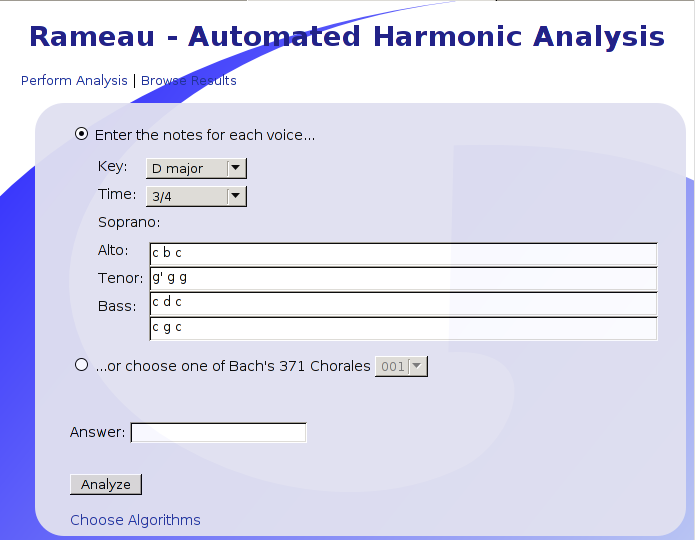
\includegraphics[scale=1]{rameau-web}
  \caption{Rameau's web interface}
  \label{fig:rameau-web}
\end{figure}

\begin{figure}
  \centering
  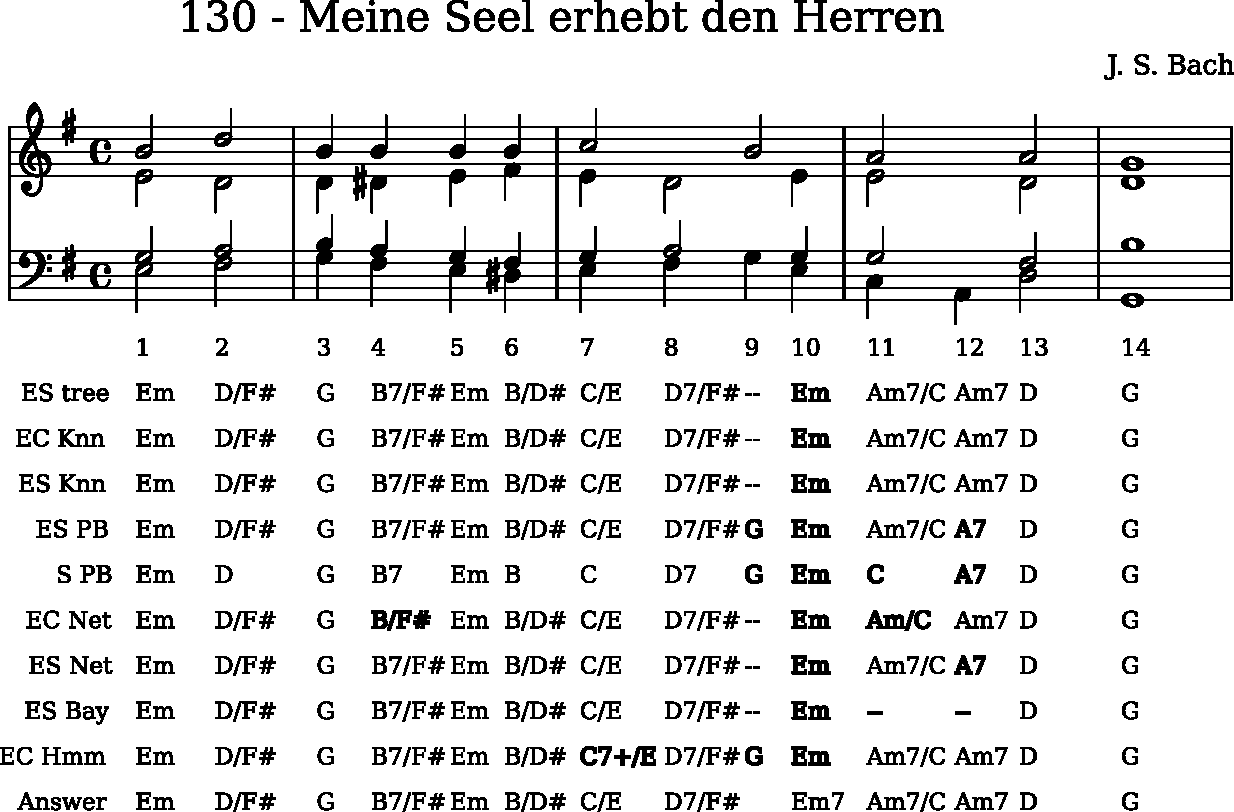
\includegraphics[scale=1]{analysis-130}
  \caption{Chord name analysis}
  \label{fig:chord-name-analysis}
\end{figure}
\begin{figure}
  \centering
  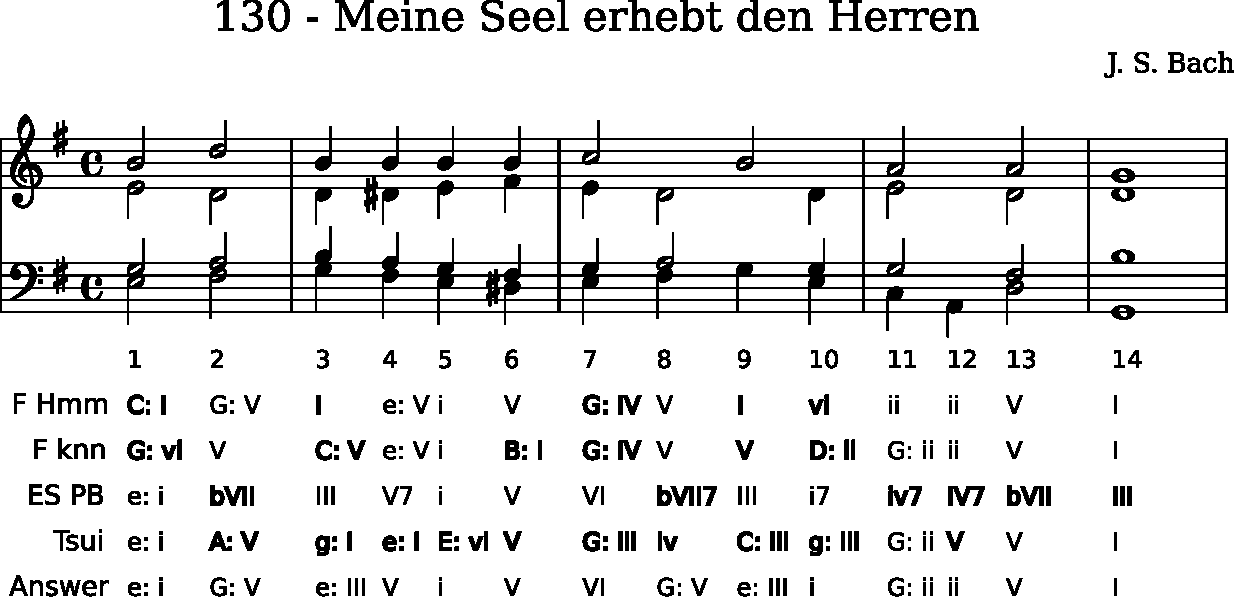
\includegraphics[scale=1]{analysis-functional-130}  
  \caption{Roman numeral analysis}
  \label{fig:roman-analysis}
\end{figure}

\begin{figure}[!h]
  \centering
  \subfigure[Chorale \#244]{
    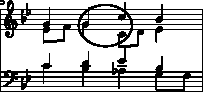
\includegraphics[scale=2]{244-oitava}
    \label{fig:244-oitava}
  }
  \qquad
  \subfigure[Chorale \#279]{
    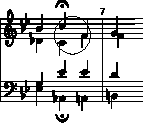
\includegraphics[scale=2]{279-oitava}
    \label{fig:279-oitava}
  }
  \qquad
  \subfigure[Chorale \#329]{
    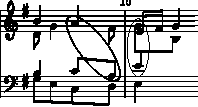
\includegraphics[scale=2]{329-oitava}
    \label{fig:329-oitava}
  }
  \caption{Consecutive octaves and unisons}
  \label{fig:oitavas-e-unissonos}
\end{figure}

\begin{table}[t]
  \centering
\begin{tabular}{l|l} \hline
 Chord type & Frequency (\%) \\ \hline
 C/F\#                & 4.2 \\
 C/D\#                & 4.2\\
 C/E                 & 4.2\\
 Cm7/C               & 4.2\\
 Cm7                 & 4.2\\
 C/B                 & 4.2\\
 Cm/C                & 4.2\\
 Cm/B                & 4.2\\
 C7                  & 4.2\\
 C7/F\#               & 8.3\\
 --                  & 8.3\\
 Cm                  &16.7\\
 C                   &29.2 \\ \hline
\end{tabular}
\caption{Chord types in in chorale \# 130}
\label{tab:ctc130}
\end{table}

\begin{figure}[!h]
  \centering
  \subfigure[Chorale \#35]{
    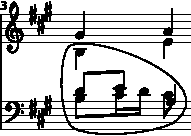
\includegraphics[scale=2]{035-16-20-cruzamento}
    \label{fig:035-cruzamento}
  }
  \subfigure[Chorale \#290]{
    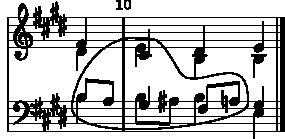
\includegraphics[scale=2]{290-66-74-cruzamento}
    \label{fig:290-66-74-cruzamento}
  }
  \caption{Voice crossing}
  \label{fig:coral-003}
\end{figure}

\begin{figure}
  \centering
  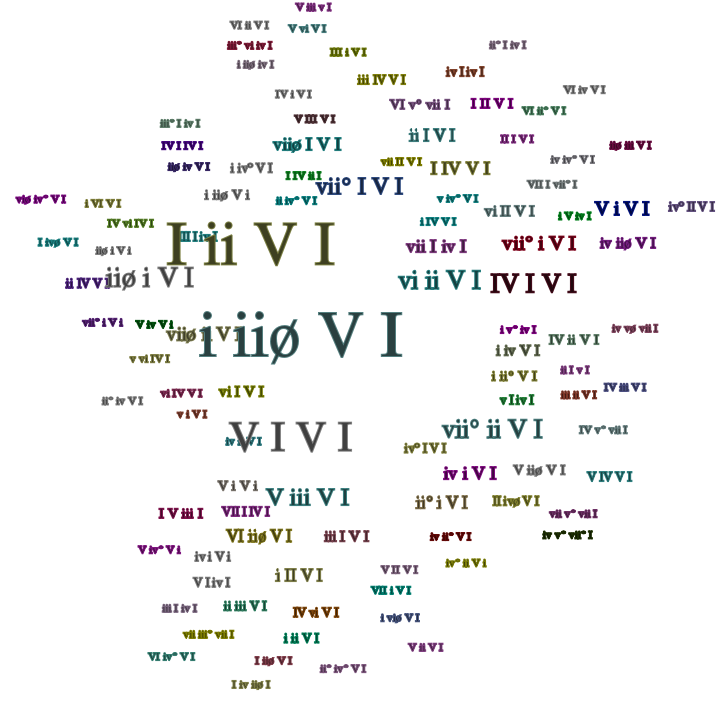
\includegraphics[scale=1]{cadences}
  \caption{Final cadences in Bach Chorales}
  \label{fig:cadences}
\end{figure}

\begin{figure}[t]
  \centering
  \includegraphics[scale=1.5,trim=0cm 5cm 0cm 2.5cm]{amostra-markov}
  \caption{A sample from the hidden Markov model}
  \label{fig:amostra}
\end{figure}

\begin{table}[h]
  \centering
  \begin{small}
    \begin{sc}
      \begin{tabular}[t]{ll} \hline
        Chord type & Notes (counting from c) \\ \hline
        Major triad & c e g \\
        Major-minor chord &  c e g b$\flat$ \\
        Minor triad & c e$\flat$ g \\
        Minor-minor chord & c $e\flat$ g b$\flat$ \\
        Fully diminished chord & c e$\flat$ g$\flat$ b$\flat\flat$ \\
        Half-diminished chord & c e$\flat$ g$\flat$ b$\flat$ \\
        Diminished triad & c e$\flat$ g$\flat$ \\
        Major-major chord & c e g b \\
        Augmented triad & c e g$\sharp$ \\
        German sixth  & c e g a$\sharp$ \\
        Italian sixth & c e a$\sharp$ \\
        French sixth & c e f$\sharp$ a$\sharp$ \\ \hline
      \end{tabular}
    \end{sc}
  \end{small}
  \caption{Templates for the Pardo \& Birmingham algorithm.}
  \label{tab:templates-pardo}
\end{table}
\end{center}

\end{multicols}

\end{document}